%% Author_tex.tex
%% V1.0
%% 2012/13/12
%% developed by Techset
%%
%% This file describes the coding for rsproca.cls

\documentclass[]{cik}%%%%where rsos is the template name



\usepackage[T1]{fontenc}
\usepackage[utf8]{inputenc}

% Pandoc citation processing
\newlength{\csllabelwidth}
\setlength{\csllabelwidth}{3em}
\newlength{\cslhangindent}
\setlength{\cslhangindent}{1.5em}
% for Pandoc 2.8 to 2.10.1
\newenvironment{cslreferences}%
  {}%
  {\par}
% For Pandoc 2.11+
\newenvironment{CSLReferences}[3] % #1 hanging-ident, #2 entry spacing
 {% don't indent paragraphs
  \setlength{\parindent}{0pt}
  % turn on hanging indent if param 1 is 1
  \ifodd #1 \everypar{\setlength{\hangindent}{\cslhangindent}}\ignorespaces\fi
  % set entry spacing
  \ifnum #2 > 0
  \setlength{\parskip}{#2\baselineskip}
  \fi
 }%
 {}
\usepackage{calc} % for calculating minipage widths
\newcommand{\CSLBlock}[1]{#1\hfill\break}
\newcommand{\CSLLeftMargin}[1]{\parbox[t]{\csllabelwidth}{#1}}
\newcommand{\CSLRightInline}[1]{\parbox[t]{\linewidth - \csllabelwidth}{#1}}
\newcommand{\CSLIndent}[1]{\hspace{\cslhangindent}#1}

\usepackage{caption}
\usepackage{booktabs}
\usepackage{longtable}
\usepackage{array}
\usepackage{multirow}
\usepackage{wrapfig}
\usepackage{float}
\usepackage{colortbl}
\usepackage{pdflscape}
\usepackage{tabu}
\usepackage{threeparttable}
\usepackage{threeparttablex}
\usepackage[normalem]{ulem}
\usepackage{makecell}
\usepackage{xcolor}

%%%% *** Do not adjust lengths that control margins, column widths, etc. ***

%%%%%%%%%%% Defining Enunciations  %%%%%%%%%%%
\newtheorem{theorem}{\bf Theorem}[section]
\newtheorem{condition}{\bf Condition}[section]
\newtheorem{corollary}{\bf Corollary}[section]
%%%%%%%%%%%%%%%%%%%%%%%%%%%%%%%%%%%%%%%%%%%%%%%

\begin{document}

%%%% Article title to be placed here
\title{The Nature of Our Literature: A Registered Report on the Positive
Result Rate and Reporting Practices in Kinesiology}

\author{
Rosie Twomey$^{1}$,
Vanessa R. Yingling$^{2}$,
Joe P. Warne$^{3, 4}$,
Christoph Schneider$^{5}$,
Chris McCrum$^{6}$,
Whitley Atkins$^{7}$,
Jenny Murphy$^{3}$,
Claudia Romero Medina$^{2}$,
Sena Harlley$^{2}$,
Aaron R. Caldwell$^{8}$}

\address{
  $^{1}$Cumming School of Medicine, University of Calgary, Calgary, AB,
Canada.\\
  $^{2}$Department of Kinesiology, California State University, East
Bay, CA, USA.\\
  $^{3}$Centre of Applied Science for Health, Technological University
Dublin, Tallaght, Dublin, Ireland.\\
  $^{4}$Setanta College, Thurles Chamber of Commerce, Tipperary,
Ireland.\\
  $^{5}$Faculty of Sport Science, Ruhr University Bochum, Bochum,
Germany.\\
  $^{6}$Department of Nutrition and Movement Sciences, NUTRIM School of
Nutrition and Translational Research in Metabolism, Maastricht
University, Maastricht, The Netherlands.\\
  $^{7}$Department of Health, Human Performance and Recreation,
University of Arkansas, Fayetteville, AR, USA.\\
  $^{8}$Society for Transparency, Openess, and Replication in
Kinesiology, Hayward, CA, USA.}
%%%% Subject entries to be placed here %%%%
\subject{
metascience}

%%%% Keyword entries to be placed here %%%%
\keywords{
Registered Report,
Metascience,
Metaresearch,
Kinesiology,
Sport and Exercise Science}

%%%% Insert corresponding author and its email address}
\corres{
  Aaron R. Caldwell\\
  {\footnotesize \href{mailto:aaron@storkinesiology.org}{\nolinkurl{aaron@storkinesiology.org}}}
}
\inserttype{
{\Large Registered Report}
}

%\insertrisenote{
%{ }
%}

\insertcite{
  Twomey et al.~(2021). The Nature of Our Literature: A Registered
  Report on the Positive Result Rate and Reporting Practices in
  Kinesiology. \textit{Communications in Kinesiology}. doi:
  10.51224/XXXXXXXXX
}

%%%% Abstract text to be placed here %%%%%%%%%%%%
\begin{abstract}
Scientists rely upon an accurate scientific literature in order to build
and test new theories about the natural world. In the past decade,
observational studies of the scientific literature have indicated that
numerous questionable research practices and poor reporting practices
may be hindering scientific progress. In particular, 3 recent studies
have indicated an implausibly high rate of studies with positive (i.e.,
hypothesis confirming) results. In Sports Medicine, a field closely
related to Kinesiology, studies that tested a hypothesis indicated
support for their primary hypothesis \textasciitilde70\% of the time.
However, a study of journals that cover the entire field of kinesiology
has yet to be completed, and the quality of other reporting practices,
such as clinical trial registration, has not been evaluated. In this
study we retrospectively evaluated 300 original research articles from
the flagship journals of North America (Medicine and Science in Sport
and Exercise), Europe (European Journal of Sport Science), and Australia
(Journal of Science and Medicine in Sport). The hypothesis testing rate
(\textasciitilde64\%) and positive result rate (\textasciitilde81\%)
were much lower than what has been reported in other fields (e.g.,
psychology), and there was only weak evidence for our hypothesis that
the positive result rate exceeded 80\%. However, the positive result
rate is still considered unreasonably high. Additionally, most studies
did not report trial registration, and rarely included accessible data
indicating rather poor reporting practices. The majority of studies
relied upon significance testing (\textasciitilde92\%), but it was more
concerning that a majority of studies (\textasciitilde82\%) without a
stated hypothesis still relied upon significance testing. Overall, the
positive result rate in kinesiology is unacceptably high, despite being
lower than other fields such as psychology, and most published
manuscripts demonstrated subpar reporting practices.
\end{abstract}
%%%%%%%%%%%%%%%%%%%%%%%%%%%

%% Some pieces required from the pandoc template
\providecommand{\tightlist}{%
  \setlength{\itemsep}{0pt}\setlength{\parskip}{0pt}}
\providecommand{\EndFirstPage}{%
}

\definecolor{jobcolor}{cmyk}{0,0,0,.95}
\definecolor{joblightcolor}{cmyk}{0,0,0,.95}
\definecolor{abstractcolor}{RGB}{207, 250, 209}
\definecolor{copyrightcolor}{RGB}{207, 250, 209}

\maketitle

\newpage

\captionsetup[table]{labelformat=empty}
\captionsetup[figure]{labelformat=empty}
\raggedbottom

\hypertarget{introduction}{%
\section{Introduction}\label{introduction}}

Scientists and knowledge-users who make decisions based on scientific
evidence rely on the published literature to be reported transparently
and to be an accurate representation of the research that scientists
conduct. The ability to replicate scientific findings is vital to
establish the credibility of scientific claims and to allow research to
progress (\protect\hyperlink{ref-NosekErrington2019}{Nosek \& Errington,
2019}). However, a large-scale collaborative effort estimated the
replicability of findings in psychological science and found that most
replication effects are smaller than originally reported
(\protect\hyperlink{ref-collaboration_estimating_2015}{Collaboration,
2015}), suggesting that our positive findings may be over-exaggerated.
Whilst this is a complex issue, questionable research practices (QRPs)
and publication bias explain some of the differences between the
original and replication effect sizes
(\protect\hyperlink{ref-head_extent_2015}{Head et al., 2015};
\protect\hyperlink{ref-John_Loewenstein_Prelec_2012}{John et al., 2012};
\protect\hyperlink{ref-simmons_false-positive_2011}{Simmons et al.,
2011}). Alongside psychology
(\protect\hyperlink{ref-collaboration_estimating_2015}{Collaboration,
2015}), other fields have struggled to replicate or reproduce findings,
including neuroscience
(\protect\hyperlink{ref-Boekel_Wagenmakers_Belay_Verhagen_Brown_Forstmann_2015}{Boekel
et al., 2015}; \protect\hyperlink{ref-Kharabian_Genon_2019}{Masouleh et
al., 2019};
\protect\hyperlink{ref-Turner_Paul_Miller_Barbey_2018}{Turner et al.,
2018}), cancer biology
(\protect\hyperlink{ref-Nosek_Errington_2017}{Nosek \& Errington,
2017}), human genetics
(\protect\hyperlink{ref-chanock_2007}{{``Replicating Genotype--Phenotype
Associations,''} 2007}) and pharmacology
(\protect\hyperlink{ref-Prinz_Schlange_Asadullah_2011}{Prinz et al.,
2011}). This type of systematic replication and evaluation of previously
published results has not yet been attempted in kinesiology
(alternatively known as sport and exercise science). However,
considering the similarities (e.g,. the study of human behavior) and
overlap (e.g.~sport and exercise psychology) between psychology and
kinesiology, we have reason to believe it may suffer from the same QRPs.
Replication appears to be rare in kinesiology, which is perhaps
surprising considering that kinesiology has been the focus of
significant critique due to overly optimistic inferences
(\protect\hyperlink{ref-Sainani_Lohse_Jones_Vickers_2019}{Sainani et
al., 2019}) and a history of underpowered studies
(\protect\hyperlink{ref-Abt_Boreham_Davison_Jackson_Nevill_Wallace_Williams_2020}{Abt
et al., 2020}). Furthermore, a lack of sample size estimation
(\protect\hyperlink{ref-Abt_Boreham_Davison_Jackson_Nevill_Wallace_Williams_2020}{Abt
et al., 2020}), misuse of p-values and statistical significance testing,
limited collaboration with statisticians
(\protect\hyperlink{ref-sainani2020}{Sainani et al., 2020}), minimal or
arbitrary use of effect sizes
(\protect\hyperlink{ref-Caldwell_Vigotsky_2020}{Caldwell \& Vigotsky,
2020}), and other reporting issues
(\protect\hyperlink{ref-Borg_Lohse_Sainani_2020}{Borg, Lohse, et al.,
2020}) appear to be commonplace.

In the past few years, a community of researchers in kinesiology have
been advocating for and adopting open and replicable research practices
(\protect\hyperlink{ref-Borg_Bon_Sainani_Baguley_Tierney_Drovandi_2020}{Borg,
Bon, et al., 2020};
\protect\hyperlink{ref-Borg_Lohse_Sainani_2020}{Borg, Lohse, et al.,
2020}; \protect\hyperlink{ref-caldwell_moving_2020}{Caldwell et al.,
2020}; \protect\hyperlink{ref-Caldwell_Vigotsky_2020}{Caldwell \&
Vigotsky, 2020}; \protect\hyperlink{ref-sainani2020}{Sainani et al.,
2020};
\protect\hyperlink{ref-Vigotsky_Nuckols_Heathers_Krieger_Schoenfeld_Steele_2020}{Vigotsky
et al., 2020}). Some journals in the field have started to adopt the
Registered Report format for manuscripts which is commendable (see
www.cos.io/rr for a list of participating journals). However, such
practices include openly sharing data and code, pre-registration, and
using the registered reports format (for a primer, see
\protect\hyperlink{ref-caldwell_moving_2020}{Caldwell et al.}
(\protect\hyperlink{ref-caldwell_moving_2020}{2020}) for details).
However, some of the issues that motivated the open science movement in
psychology and other fields
\protect\hyperlink{ref-munafo_manifesto_2017}{Munafò et al.}
(\protect\hyperlink{ref-munafo_manifesto_2017}{2017}) are comparatively
unexplored in kinesiology, and currently the number of kinesiology
researchers adopting open research practices is largely unknown. There
is some indication that both pre-registration and sharing of data is
uncommon (\protect\hyperlink{ref-Borg_Lohse_Sainani_2020}{Borg, Lohse,
et al., 2020}; \protect\hyperlink{ref-Tamminen_Poucher_2018}{Tamminen \&
Poucher, 2018}) and flagship journals of our field (e.g., Medicine \&
Science in Sport \& Exercise, European Journal of Sport Science) do not
include a statement encouraging open data availability in the author
guidelines (Oct 2020). Evaluating a recent sample of the kinesiology
literature for such practices may help draw attention to these potential
issues.

Another issue that warrants consideration is the positive result rate
(the rate at which a published study finds support for its hypothesis)
of published kinesiology studies. Recently,
\protect\hyperlink{ref-buttner_2020}{Büttner et al.}
(\protect\hyperlink{ref-buttner_2020}{2020}) estimated the positive
result rate in three high ranking sports journals and one high ranking
sports physiotherapy journal. In line with previous research in other
scientific disciplines
(\protect\hyperlink{ref-fanelli_positive_2010}{Fanelli, 2010};
\protect\hyperlink{ref-scheel_excess_2020}{Scheel et al., 2021}), the
positive result rate exceeded 80\%. What are the mechanisms for the
suspiciously high positive result rates in the scientific literature?
Given the assumption of a completely unbiased literature, such a high
positive result rate could only occur if both statistical power and the
proportion of true hypotheses that researchers have chosen to test is
consistently high \protect\hyperlink{ref-scheel_excess_2020}{Scheel et
al.} (\protect\hyperlink{ref-scheel_excess_2020}{2021}). The more
plausible explanation perhaps, corroborated in previous work
(\protect\hyperlink{ref-John_Loewenstein_Prelec_2012}{John et al.,
2012}; \protect\hyperlink{ref-simmons_false-positive_2011}{Simmons et
al., 2011}), is that the literature is distorted by undisclosed
flexibility in analysis and other QRPs, and the incentive to publish
positive results. Registered reports are specifically designed to help
mitigate these issues
\protect\hyperlink{ref-chambers_registered_2015}{Chambers et al.}
(\protect\hyperlink{ref-chambers_registered_2015}{2015}). Therefore,
\protect\hyperlink{ref-scheel_excess_2020}{Scheel et al.}
(\protect\hyperlink{ref-scheel_excess_2020}{2021}) assessed the positive
result rate in research articles published using the traditional format
in comparison to registered reports in a sample of the psychology
literature. The positive result rate was an implausibly high 96\% for
traditional articles and a significantly lower 46\% for registered
reports. The increased methodological rigour inherent to the registered
report format has clearly led to an increase in the reporting of null
findings in the psychological literature.

The equivalent findings regarding standard and registered reports have
not been reported for kinesiology, and simply would not be possible
given the current literature; unlike psychological science
(\protect\hyperlink{ref-scheel_excess_2020}{Scheel et al., 2021}), and
to our knowledge, kinesiology has not accumulated more than 70
registered reports to evaluate against traditional publication formats.
The adoption of registered reports in kinesiology is progressing slowly.
One reason for this may be a lack of awareness regarding the replication
crisis and movement towards more rigorous and transparent research
practices. However, the slow adoption of registered reports could also
be due to a lack of concern about the kinesiology literature given the
limited evidence exploring these potential issues in our field.

The primary aim of this study was to assess the positive result rate of
reported hypotheses in the recent kinesiology literature, using
society-affiliated flagship journals from the field. Considering the
majority of scientific disciplines documented by
\protect\hyperlink{ref-fanelli_how_2009}{Fanelli}
(\protect\hyperlink{ref-fanelli_how_2009}{2009}) had a positive rate of
80\%, we hypothesized that the \(>\) 80\% of the published studies in
kinesiology would report positive results (i.e, support for the
hypothesis) for their first stated hypothesis. Our secondary aims were
to assess a number of related research practices, including whether the
kinesiology literature includes replications of previous effects, the
detail of statistical reporting and adoption of other transparent
reporting practices.

\hypertarget{methods}{%
\section{Methods}\label{methods}}

\hypertarget{sample}{%
\subsection{Sample}\label{sample}}

Research articles were sampled from three flagship kinesiology journals:
Medicine and Science in Sport and Exercise (MSSE), the European Journal
of Sport Science (EJSS) and the Journal of Science and Medicine in Sport
(JSAMS), which represent three major kinesiology societies of North
America (American College of Sports Medicine), Europe (European College
of Sport Science) and Australia (Sports Medicine Australia),
respectively. We selected three major societies and their official
flagship journals because we believed they represent a diverse selection
of research in kinesiology and provide insights into the practices of
the field as a whole. In addition, we chose to focus on these three
journals rather than a random sample of the entire literature because
these journals should represent the best research in the field (compared
to any published article which could be sampled from a possible
predatory publisher). We selected 100 original research articles per
journal, 300 in total, excluding study protocols, methodological
tutorials/reports, opinions, commentaries, perspectives, conference
proceedings, narrative reviews, systematic reviews and meta-analyses. We
also excluded research articles if they have been retracted or contained
insufficient information to reach coding decisions (none were observed
in the current study). To sample a recent selection of the literature,
research articles were sampled consecutively backwards from December 31,
2019, by the data analyst (ARC) until 100 were included for each
journal.

\hypertarget{data-extraction}{%
\subsection{Data Extraction}\label{data-extraction}}

We identified nine coders who were responsible for data extraction.
Coders underwent standardized training that has been designed based on
the queries raised and clarification required during pilot testing (see
later section). These nine coders formed three teams of three, and each
team was allocated the research articles from one journal (MSSE, EJSS,
or JSAMS). All coders extracted data independently and entered this
directly into a Qualtrics survey. The Qualtrics survey was refined after
pilot testing and a copy can be found at our Open Science Framework
repository (see \protect\hyperlink{data}{Data Accessibility} statement).
Each team was coordinated by a team leader trained at a doctoral level
in a kinesiology discipline (RT, VY and JW). Once independent coding was
complete, interrater reliability was assessed using Fleiss's Kappa. Team
leaders were responsible for resolving all conflicts (any instance where
there was not agreement between all group members) within their team
through group review of the item and group discussion. Where conflicts
could not be resolved (and revised if necessary) using this process, the
team leader consulted the other two team leaders. All data (original
coder responses and summary decisions) is available on study's Open
Science Framework repository (see \protect\hyperlink{data}{Data
Accessibility} statement).

\hypertarget{measures-and-coding-procedure}{%
\subsection{Measures and Coding
Procedure}\label{measures-and-coding-procedure}}

All articles were categorized as basic physiology (animal and cell
physiology), applied exercise physiology (human), environmental
physiology (heat, cold, and altitude), clinical research, biomechanics,
motor learning/control/behavior, epidemiology, sport/exercise
psychology, sport performance, or other (the category that best
describes the article). Only research articles that included explicit
statements that a hypothesis was tested were included in the analysis of
the positive result rate. However, all articles (i.e., 300) were
included in analysis related to replication status, statistical
reporting and other reporting practices, as described in the following
sections.

\hypertarget{support-for-a-hypothesis-in-the-kinesiology-literature}{%
\subsection{Support for a Hypothesis in the Kinesiology
Literature}\label{support-for-a-hypothesis-in-the-kinesiology-literature}}

From the 300 articles, we expected that approximately 60\% would include
explicit statements that a hypothesis was tested as part of the study
(e.g., ``We hypothesized that\ldots{}'')
(\protect\hyperlink{ref-buttner_2020}{Büttner et al., 2020}). Therefore,
we expected to extract data on the positive results rate from
approximately 180 research articles. The main dependent variable was
whether the \emph{first} stated hypothesis was supported or not, as
reported by the authors. We planned to closely follow the coding
procedure used by \protect\hyperlink{ref-fanelli_positive_2010}{Fanelli}
(\protect\hyperlink{ref-fanelli_positive_2010}{2010}) and
\protect\hyperlink{ref-scheel_excess_2020}{Scheel et al.}
(\protect\hyperlink{ref-scheel_excess_2020}{2021}), which is described
as follows: By examining the abstract and/or full text, it will be
determined whether the authors of each paper had concluded to have found
a positive (full or partial) or negative (null or negative) support. If
more than one hypothesis was being tested, only the first one to appear
in the text was considered. The coding of support for the hypothesis was
based on the author's description of their results. In line with
previous work (\protect\hyperlink{ref-buttner_2020}{Büttner et al.,
2020}; \protect\hyperlink{ref-scheel_excess_2020}{Scheel et al., 2021}),
we coded a hypothesis as having received ``support,'' ``partial
support,'' ``no support'' or ``unclear or not stated.'' We added this
fourth option after pilot indicated that some authors failed to state
whether or not the study's hypotheses were, or were not, supported in
the discussion section of the manuscript. This was re-coded into a
binary ``support'' (full or partial) vs.~``no support'' variable, with
``unclear or not stated'' removed, for the main analysis. The language
used to state a hypothesis and support for the first tested hypothesis
were included in the data extraction and are included in the final
dataset.

\hypertarget{replication-status}{%
\subsection{Replication Status}\label{replication-status}}

Coders assessed whether a study is a replication of a previously
published one, as reported by the authors. Coders searched the full
texts of all papers for the string `replic*' and, for papers that
contained it, indicated whether the coded hypothesis was a close
replication with the goal to verify a previously published result
(\protect\hyperlink{ref-scheel_excess_2020}{Scheel et al., 2021}).

\hypertarget{statistical-reporting}{%
\subsection{Statistical Reporting}\label{statistical-reporting}}

Coders assessed whether authors included language related to statistical
significance and if p-values were included in the results (relating to
all analyses and not only the first hypothesis). If yes, coders assessed
if the p-value was interpreted as significant and if the exact or
relative p-value was reported (i.e., p=0.049 vs.~p\textless0.05). If a
relative p-value was reported, the level of the reported p-value (e.g.,
p\textless0.05, p\textless0.01) were coded. But a ``p\textless0.001''
was considered exact since some statistical software does not provide
p-values less than this threshold. This decision was made by team
leaders after disagreements in the coding process. Coders also extracted
whether an effect size was reported at any stage of the manuscript,
including, but not limited to: Cohen's d, correlation coefficients, mean
differences, and measures of model fit (e.g., coefficient of
determination: \(R^2\)). Coders assessed whether the information on
sample size was provided, and if provided, the total sample size (the
number of participants included in the analyses, rather than the planned
sample size) will be extracted. Also, coders assessed whether any sample
size justification (e.g.~power analysis) were included in the
manuscript.

\hypertarget{other-reporting-practices}{%
\subsection{Other Reporting Practices}\label{other-reporting-practices}}

Coders assessed whether the study was a clinical trial, according to the
International Committee of Medical Journal Editors (ICMJE) definition of
\href{http://www.icmje.org/recommendations/browse/publishing-and-editorial-issues/clinical-trial-registration.html}{clinical
trials} (\protect\hyperlink{ref-icmje}{{``Clinical Trials,''} 2021}). If
yes, coders assessed if a clinical trial registration was reported in
the manuscript. For all other types of studies, coders assessed whether
studies were pre-registered (as reported within the manuscript).
Additionally, the coders indicated if a study was a randomized control
trial (RCT) or was a study involving animal models. Coders assessed if a
manuscript provided a statement on original data availability (not
\emph{additional} supplementary data), and, if yes, whether there was
open access to the original data and/or code via a link or supplementary
file.

\hypertarget{pilot-testing}{%
\subsection{Pilot Testing}\label{pilot-testing}}

To ensure that our questionnaire for our raters accurately and
consistently reflected the above-detailed information from relevant
articles, we conducted pilot testing before submission of the Stage 1
manuscript. Fifteen original research articles published in 2018, five
from each of our three chosen journals, were selected to be used for
pilot testing. One team of naive coders (i.e., were not trained prior to
coding) extracted all data from these articles and entered this into
Qualtrics. Independent coding was checked for disagreements, and this
was used to inform training procedures. Pilot aggregated data were
generated, and further adjustments were made to refine the planned
extraction and analysis process. A summary report of the pilot work can
be found on our \protect\hyperlink{data}{data repository}. Overall, our
pilot work indicated minimally acceptable agreement among the raters on
the questions essential to our study such as whether a hypothesis was
tested (\(\kappa\) = 0.903; complete agreement = 14/15) and if the
authors found support for this hypothesis (\(\kappa\) = 0.586; complete
agreement = 6/9). For all items with rater disagreement, at least two
coders were in agreement on the rating. After the conclusion of pilot
testing, a forum among the team was completed in order to appropriately
adjust the questionnaire and refine future instructions/training for the
coding teams in the full study. Prior to coding, all coding team members
underwent formal training and were presented with example articles (not
from the study sample) in order to improve consistency in the coding
process.

\hypertarget{statistical-analysis}{%
\subsection{Statistical Analysis}\label{statistical-analysis}}

A detailed summary of the planned hypothesis test, ``power'' analysis,
inter-rater reliability, and final analyses (code included) can be found
at our Open Science Framework \protect\hyperlink{data}{repository}.
Additional data related to the inter-rater reliability can be found
within the supplemental material.

\hypertarget{confirmatory-analyses}{%
\subsubsection{Confirmatory Analyses}\label{confirmatory-analyses}}

First, we estimated the rate at which kinesiology research finds support
for the first tested hypothesis (as reported by the authors). Further,
we planned to compare this to the majority of disciplines surveyed in
\protect\hyperlink{ref-fanelli_positive_2010}{Fanelli}
(\protect\hyperlink{ref-fanelli_positive_2010}{2010}) which reported a
positive result rate in excess of 80\% (16 of 20 disciplines). We
believed it unlikely that kinesiology would have a positive result rate
lower than 80\%, and believe that the actual rate is closer to the
social sciences at approximately 85\%
(\protect\hyperlink{ref-fanelli_positive_2010}{Fanelli, 2010}).
Considering we had prior information, and a belief we wanted to test, we
opted to use a Bayesian analysis to test our hypothesis. Therefore, we
planned to test our hypothesis that the positive result rate is greater
than 80\% using a generalized Bayesian regression model
(\protect\hyperlink{ref-Burkner_2017}{Bürkner, 2017}). We assumed a
prior of \(\beta(17,3)\) on the intercept of the model (i.e., the rate
of positive results). Evidence for our hypothesis is reported as the
posterior probability, \(pr(Intercept > .8 | data)\), of our hypothesis
and the Bayes Factor (BF), the ratio of evidence for our hypothesis
versus the null (i.e., \(H_0: \theta \le 0.8\)). We performed a Monte
Carlo simulation assuming we obtained 150 studies which contained
hypotheses from a population where 85\% will contain a positive result
for the first stated hypothesis. This simulation indicated that our
model would have an 87\% chance of being able to obtain some evidence
(BF in favor of our hypothesis \(>\) 3) for our hypothesis.

\hypertarget{exploratory-analyses}{%
\subsubsection{Exploratory Analyses}\label{exploratory-analyses}}

Sample sizes were compared between disciplines using a one-way Analysis
of Variance (ANOVA). Due to the skew in the reported sample sizes, a
natural log transformation was applied to the reported sample size to
improve model fit and reduce heteroscedasticity. Partial eta-squared
(\(\eta^2_{p}\)) is reported alongside the F-test for this analysis as a
measure of effect size. All other data is summarized descriptively and
as frequencies and proportions with Pearson's \(\chi^2\)
(\texttt{chisq.test} in R) and binomial (\texttt{binom.test} in R)
proportions tests where appropriate. Brackets indicate a 95\%
compatibility interval (confidence or posterior for the frequentist and
Bayesian approaches respectively). For the frequentist analyses, we did
not set an \emph{a priori} significance cutoff, and applied an
``unconditional'' analysis of these results
(\protect\hyperlink{ref-rafi2020semantic}{Rafi \& Greenland, 2020}).

\hypertarget{results}{%
\section{Results}\label{results}}

\hypertarget{confirmatory-results}{%
\subsection{Confirmatory Results}\label{confirmatory-results}}

There was weak support for our hypothesis that manuscripts would find
some support for their hypothesis 80\% of the time. There was only a
70.82\% posterior probability of our hypothesis with it being 2.43 times
more likely than the null hypothesis. However, the data did favor our
secondary hypothesis that at least 60\% of manuscripts perform
hypothesis testing with it being 9.72 times more likely than the null
(Posterior Probability: 90.67\%). Overall, we estimate that the positive
result rate is 81.43\% {[}75.78, 86.3{]}, and there is a 63.58\%
{[}58.12, 68.97{]} rate of hypotheses being tested in manuscripts
(Figure 1A). Interestingly, we did find a substantial rate (6.8\%) of
manuscripts not reporting whether or not a hypothesis was supported
(Figure 1B).

\begin{figure}[H]
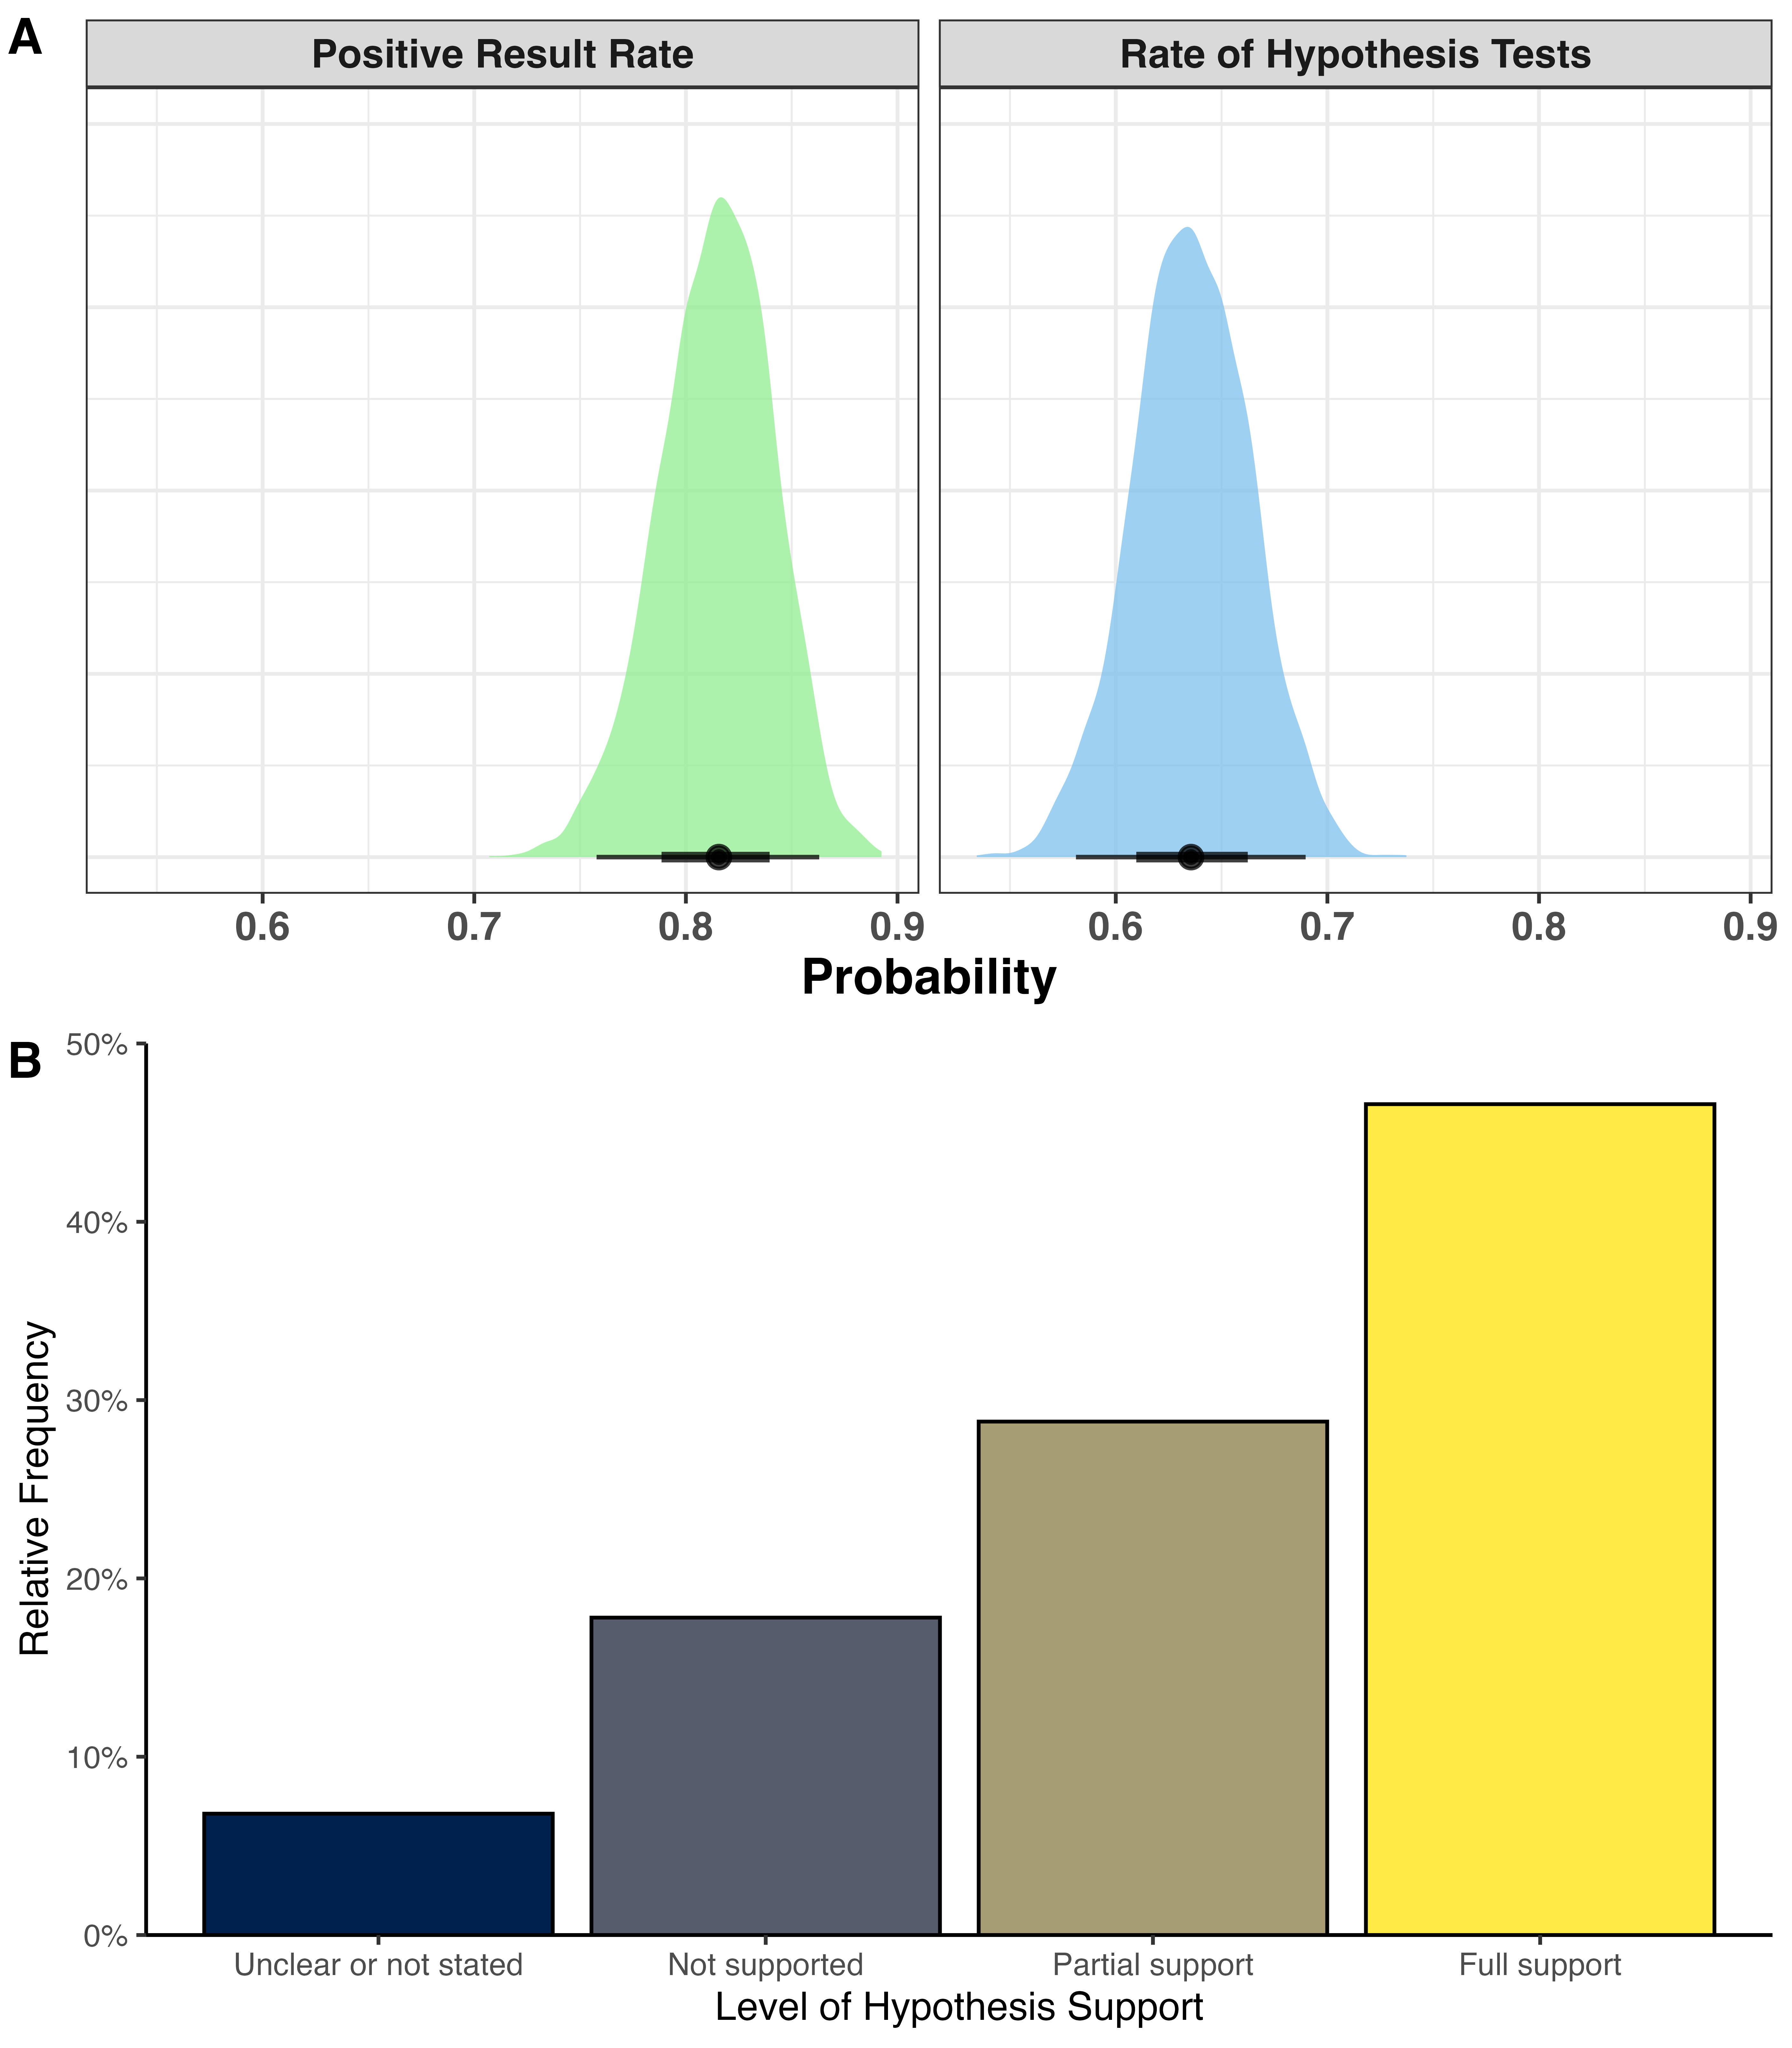
\includegraphics[width=0.9\linewidth]{figure1} \caption{Figure 1. A) Posterior distributions from Bayesian model with the 50\% and 95\% percent compatibility intervals represented by the error bars at the bottom and B) Relative frequencies of the level of support reported for manuscripts with  a hypothesis (N = 191) with 17.8\% report no support, 28.8\% stating partial support, 46.6\% stating full support, and  6.81\% for which support was unclear or not stated.}\label{fig:fig1}
\end{figure}

\newpage

\hypertarget{exploratory-results}{%
\subsection{Exploratory Results}\label{exploratory-results}}

\hypertarget{statistics-reporting}{%
\subsubsection{Statistics Reporting}\label{statistics-reporting}}

Nearly all manuscripts, 90\% {[}86.03, 93.15{]}, reported some form of
significance testing. Even when a hypothesis was not stated or tested,
significance testing was utilized in 81.65\% {[}73.09, 88.42{]} of
manuscripts (89 of the 109 manuscripts without a stated hypothesis).
Most manuscripts, 79.33\% {[}74.3, 83.77{]}, also reported some form of
effect size to accompany the results. In addition, 33.7\% {[}28.09,
39.68{]} of manuscripts reported exact p-values for all results (e.g.,
p=0.045) versus only relative p-values (e.g., p\textless0.05). Though,
89.63\% {[}85.36, 93{]} of manuscripts reported at least \emph{some}
exact p-values (e.g., p=0.045) versus relative p-values (e.g.,
p\textless0.05), and therefore changed their reporting method within the
paper by switching between exact and relative p-values.

\hypertarget{other-important-reporting-practices}{%
\subsubsection{Other Important Reporting
Practices}\label{other-important-reporting-practices}}

Registration or preregistration of studies was low with 9\% {[}6.01,
12.82{]} of manuscripts reporting preregistration or clinical trial
registration information. Sample size information was often well
reported, with 97.67\% {[}95.25, 99.06{]} of manuscripts reported all
the required sample size information (total and group sample sizes).
However, sample size justification information (e.g., power analysis)
only appeared in 22.67\% {[}18.05, 27.83{]} of manuscripts. None of the
manuscripts analyzed for this study were considered a replication
attempt by the original study authors. Only 2.33\% {[}0.94, 4.75{]} of
manuscripts had a data accessibility statement. Further, 0.67\% {[}0.08,
2.39{]} of manuscripts reported some form of data sharing or open data.

\hypertarget{analysis-by-journal}{%
\subsubsection{Analysis by Journal}\label{analysis-by-journal}}

We tested for differences in the degree of support for the first stated
hypothesis between the three journals, but no differences were noted,
\(\chi^2\)(6) = 2.4; p=0.879, (Figure 2B). All three journals had ``Full
support'' for the stated hypothesis in \textgreater45\% of manuscripts.
However, there were clear differences, \(\chi^2\)(2) = 20.43;
p\textless0.001, in the rate of hypotheses being tested (Figure 2A). The
majority of MSSE and EJSS had hypothesis tests (74\% and 71\%
respectively), but JSAMS had a much lower rate of hypothesis tests
(46\%). An effect size was often reported in manuscripts, but EJSS
(90\%) had a much better reporting rate, \(\chi^2\)(2) = 10.9; p=0.004,
compared to JSAMS (72\%) or MSSE (76\%; Figure 2C). While sample size
justifications were rare (Figure 2D), MSSE (35\%) had a higher rate of
reporting a sample size justification, \(\chi^2\)(2) = 13.73; p=0.001,
compared to EJSS (19\%) or JSAMS (14\%). The rate of reporting
significance tests in all journals was high (\textgreater{} 80\%).
However, JSAMS (84\%) reported a slightly lower rate of significance
tests, \(\chi^2\)(2) = 6.22; p=0.045, than EJSS (92\%) or MSSE (94\%).

\newpage

\begin{figure}[H]
\includegraphics[width=0.5\linewidth]{figure2} \caption{Figure 2. Relative frequencies, by journal, for A) level of reported support for a hypothesis, B) indication of whether a hypothesis was tested, C) indication of whether an effect size was reported, or D) indication of if sample size was justified by the authors. Journals included the European Journal of Sport Science (EJSS), the Journal of Science and Medicine in Sport (JSAMS), and Medicine and Science in Sport and Exercise (MSSE), }\label{fig:fig2}
\end{figure}

\newpage

\hypertarget{analysis-by-discipline}{%
\subsubsection{Analysis by Discipline}\label{analysis-by-discipline}}

When comparing between disciplines, we observed a large variation in the
degree of support found for the proposed hypothesis, \(\chi^2\)(27) =
40.02; p=0.051. In fact, motor behavior and environmental physiology
studies all found full or partial support within the sample of
manuscripts (Figure 3B). Basic physiology was the worst at not reporting
whether or not a hypothesis was supported with 37.5\% of the studies
never making a clear statement of support (Figure 3B). The rate of
hypothesis testing differed greatly between disciplines, \(\chi^2\)(9) =
28.44; p\textless0.001 (Figure 3A). The extremes of the spectrum ranged
from epidemiology (25.9\%) to basic physiology (88.9\%). Sample size,
evaluated using a linear model with a natural log transformation of the
total sample size, differed between disciplines, F(9, 285) = 21.81,
p=\(2.2 \cdot 10^{-16}\), \(\eta^2_g\) = 0.408. The estimated average
sample size, derived from the estimated marginal mean, per discipline
ranged from the lowest in environmental physiology, N = 16 {[}7, 37{]},
to the highest in epidemiology, N = 1162 {[}691, 1952{]} (Figure 2C).

\newpage

\begin{figure}[H]
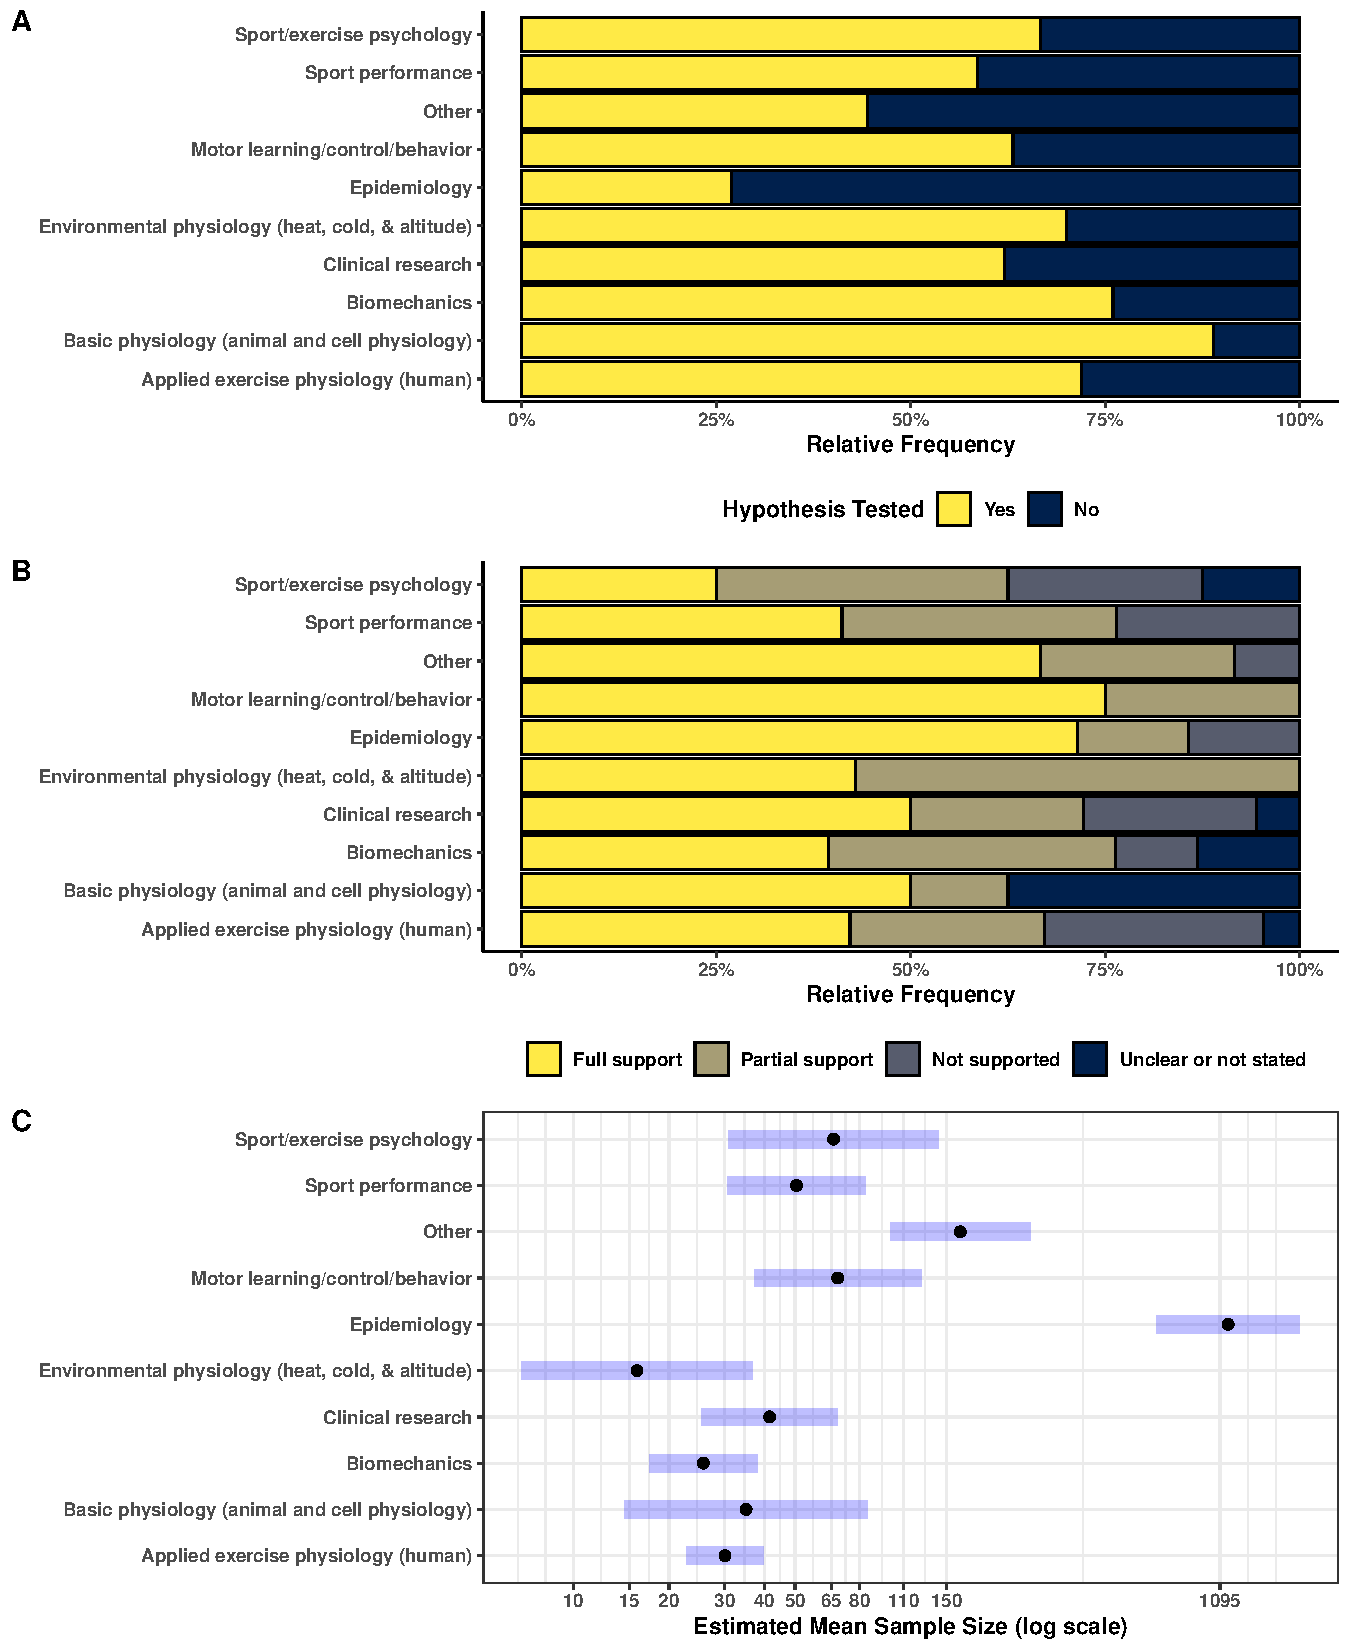
\includegraphics[width=0.9\linewidth]{figure3} \caption{Figure 3. The breakdown, by discipline, for A) indication of whether a hypothesis was tested B) level of reported support for a hypothesis,  and C) the estimated total sample size (grey bands indicate 95\% confidence intervals).}\label{fig:fig3}
\end{figure}

\newpage

\hypertarget{analysis-of-clinical-and-randomized-control-trials}{%
\subsubsection{Analysis of Clinical and Randomized Control
Trials}\label{analysis-of-clinical-and-randomized-control-trials}}

Clinical trials (N = 40) had lower rates of reported support for the
hypothesis, 64\% {[}42.5, 82{]}, but similar hypothesis testing rates,
67.5\% {[}50.8, 81.4{]}, compared to the rest of the analyzed
manuscripts. Despite guidelines strongly recommending sample size
justifications, only 62.5\% {[}45.8, 77.3{]} reported a sample size
justification within the manuscript. In addition, despite regulations
that require clinical trial registration
(\protect\hyperlink{ref-clinreg2016}{Health \& Services, 2016}), only
57.5\% {[}40.9, 72.9{]} reported clinical trial registration or
preregistration documentation.

Another category of studies that requires particular reporting are RCTs
(N = 64). Overall, the manuscripts including RCTs had similar rates of
supporting the hypothesis, 75\% {[}59.7, 86.8{]} and a slightly higher
estimated rate, 73.4\% {[}60.9, 83.7{]}, of testing hypotheses. Like
clinical trials, RCTs often lacked sample size justifications, 50\%
{[}37.2, 62.8{]}, and lacked pre-registrations, 28.1\% {[}17.6, 40.8{]}.

\hypertarget{discussion}{%
\section{Discussion}\label{discussion}}

We performed a systematic evaluation of the 300 journal articles
published in the flagship journals of three major sport and exercise
science societies. Our primary hypothesis that the proportion of studies
finding support for their first hypothesis would be more than 80\% was
weakly corroborated. This positive result rate is still excessively high
at 81\%, and would likely be much lower with more stringent criteria for
hypothesis tests. Our secondary hypothesis that more than 60\% of
articles would explicitly report a hypothesis was corroborated, though
our estimate of approximately 64\% is relatively low when considering
that \textgreater90\% of articles used null hypothesis significance
testing. The combination of the low proportion of null results, lack of
sample size justifications, low numbers of pre-registrations (even in
the case of clinical trials), the near absence of open data, and the
complete absence of replication studies compromises the credibility of
kinesiology as field of scientific research.

The positive result rate observed in this study is very similar to what
has been observed in a variety of other fields. In a recent study of
sports medicine, \protect\hyperlink{ref-buttner_2020}{Büttner et al.}
(\protect\hyperlink{ref-buttner_2020}{2020}) estimated the positive
result at \textasciitilde82.2\%
(\protect\hyperlink{ref-buttner_2020}{Büttner et al., 2020}) which is
almost indistinguishable from the estimated rate in our study of
kinesiology (\textasciitilde81\%; Figure 1A). However, the positive
result rates for kinesiology and sports medicine are slightly lower than
the overall scientific positive result rate of 84\% reported by
\protect\hyperlink{ref-fanelli_positive_2010}{Fanelli}
(\protect\hyperlink{ref-fanelli_positive_2010}{2010}). The positive
result rate does appear to vary by field with some fields having
positive result rates as low as 70\% (space science) and as high as 90\%
(psychology) (\protect\hyperlink{ref-fanelli_positive_2010}{Fanelli,
2010}). The results from our study and
\protect\hyperlink{ref-buttner_2020}{Büttner et al.}
(\protect\hyperlink{ref-buttner_2020}{2020}) would place kinesiology and
sports medicine closer to the ``hard'' sciences than to the ``soft''
sciences (\protect\hyperlink{ref-fanelli_positive_2010}{Fanelli, 2010}).
The positive result rate in kinesiology is almost certainly lower than
psychology which is estimated to report support for hypotheses in
\textasciitilde96\% of manuscripts involving original research
(\protect\hyperlink{ref-scheel_excess_2020}{Scheel et al., 2021}).
However, the positive result rate in kinesiology is still unreasonably
high, and efforts to reduce the positive result rate should be
undertaken. As \protect\hyperlink{ref-scheel_excess_2020}{Scheel et al.}
(\protect\hyperlink{ref-scheel_excess_2020}{2021}) demonstrated, when
researchers adopt a registered report approach the positive result rate
drops to 46\%.

In the current study, we observed that \textasciitilde60\% of
manuscripts reported that they were testing hypotheses, and this is
almost identical to the rate reported by
\protect\hyperlink{ref-buttner_2020}{Büttner et al.}
(\protect\hyperlink{ref-buttner_2020}{2020}). As
\protect\hyperlink{ref-fanelli_positive_2010}{Fanelli}
(\protect\hyperlink{ref-fanelli_positive_2010}{2010}) noted, researchers
may selectively report whether or not hypothesis testing was the
original goal of a study. Some researchers may have removed language
regarding hypothesis testing if their planned hypothesis did not get the
support they were expecting, or if the results were ambiguous.
Approximately 80\% of the studies within our study that did not report a
hypothesis utilized significance testing, which is a statistical tool
intended for testing hypotheses. Therefore, we believe it is possible
that some studies included in our sample may have originally been
intended to test hypotheses but the language regarding hypothesis tests
was removed during the writing process. If studies and hypotheses were
pre-registered, or written as a registered report, then the positive
result rate may have been lowered simply due to the fact that language
regarding hypothesis tests would still be included within the
manuscript.

Assuming no bias in the scientific record, the positive result rate of a
sample of articles would depend on the statistical power and proportion
of true hypotheses tested in the included studies
(\protect\hyperlink{ref-ioannidis_why_2005}{Ioannidis, 2005};
\protect\hyperlink{ref-scheel_excess_2020}{Scheel et al., 2021}). The
proportion of true hypotheses being tested may be higher in kinesiology
compared to fields like psychology
(\protect\hyperlink{ref-scheel_excess_2020}{Scheel et al., 2021}).
Kinesiology studies can be demanding or invasive for participants and
resource-intensive due to the use of specialist equipment, techniques,
or the time and personnel required for specific study designs (for
example, training studies with multiple laboratory visits). Therefore,
kinesiology researchers may design studies to test trivial hypotheses
where a positive result is largely foreseeable (and potentially
unimportant) in order to increase the odds of ``success'' when resources
are constrained. Arguably, a resource-intensive discipline is
environmental physiology (e.g., studies in this field may require
environmental chambers that cost hundreds of thousands of dollars and
limit data collection to 1 participant per day), and, in our sample,
100\% of these studies found some support for their hypothesis. However,
we find it unlikely that such a high rate of true hypotheses in the
literature explains the high positive result rate because this also
depends on the vast majority of studies having high statistical power
(\textasciitilde80\%). Less than 25\% of the articles in our sample
included a sample size justification, so for the vast majority of
articles testing a hypothesis, the statistical power and effect size
calculated during study design (if a power analysis was performed) were
unknown. Although the proportion of sample size justifications was
higher in MSSE (35\%), this is underwhelming considering their
guidelines ask authors to justify the adequacy of their sample size by
reporting the results of power calculations for the main statistical
test(s).

Based on median sample sizes of 73-183,
\protect\hyperlink{ref-fraley2014}{Fraley \& Vazire}
(\protect\hyperlink{ref-fraley2014}{2014}) found that typical studies
published in top psychology journals do not have adequate power (50\%)
to detect typical effect sizes (d=0.4). In contrast, we estimated sample
sizes below 40 for many (4 of 10) sub-disciplines and below 70 for all
but two sub-disciplines (i.e., ``other'' and epidemiology; Figure 3C).
Comparing these smaller sample sizes to those in psychology, we consider
it unlikely that the typical studies published in our kinesiology
society journals have high statistical power. This seems even more
unrealistic for environmental physiology, considering an estimated
median sample size of 16. The problem of underpowered studies in our
field has previously been raised by
\protect\hyperlink{ref-knudson2017}{Knudson}
(\protect\hyperlink{ref-knudson2017}{2017}), who highlighted typically
small sample sizes (median 12-18) and biased effects in applied
biomechanics journals. Similar concerns about imprecise studies have
also been raised for the Journal of Sports Science, where the median
sample size was 19 (\protect\hyperlink{ref-abt2021}{Abt et al., 2021}).
This issue is compounded when small effect sizes are considered
clinically or practically important (in elite athletes or in clinical
populations, this may well be the case). With small sample sizes,
typical kinesiology studies may not be adequately powered to detect what
could be considered a meaningful effect. Therefore, rather than a
consistently high proportion of true hypotheses being tested and
consistently high statistical power, it is more reasonable to suggest
that a combination of factors including bias, convenience or limited
sampling, and QRPs may explain the excessive positive result rate in the
kinesiology literature, and this should be further investigated.

It would not be fair of us to suggest that deliberate data manipulation
is prevalent in our field; QRPs can be intentional or unintentional.
Some researchers may lack awareness and consider QRPs to be a normal
part of the research process rather than a concerted effort to produce
misleading studies. Unconscious biases may cause a tendency for
researchers to confirm tested hypotheses (confirmation bias) and can
influence participants to meet researcher expectations. In fact, many
coders made anecdotal notes that hypotheses were often so vague that
\emph{any} result could be spun to support the hypothesis. Similarly,
researchers may be aware of publication bias and may be influenced by
the perception that a compelling ``story'' will be more publishable.
Despite worldwide initiatives (\protect\hyperlink{ref-DORA2013}{Cagan,
2013}), there are also clear academic incentives for arriving at
positive results because publication quantity and journal-based metrics
can be rated above societal impact in funding, appointment, and
promotion decisions, and therefore impact career advancement. Registered
reports offer one solution because articles are peer-reviewed before
data collection, so poorly designed research, or a vague hypothesis,
does not progress to an in-principle acceptance. The registered report
format is designed to prevent several QRPs and a bias (whether from the
researchers, reviewer, or editor) towards findings that support the
hypothesis. Registered reports also prevent the findings from being
suppressed by peer reviewers (e.g., in the case that the findings refute
previous work) since an in-principle acceptance is based on the
rationale and methods alone. The effect of registered reports is clear
in psychology, where the format moves the positive result rate closer to
50\% and introduces adequately powered studies with null results into
the scientific record (\protect\hyperlink{ref-scheel_excess_2020}{Scheel
et al., 2021}). This data is then available to other researchers rather
than being consigned to the ``file drawer'' (an analogy for a
researcher's negative results that were either not submitted or not
accepted for publication), who may have otherwise wasted valuable
resources towards testing a hypothesis that may be false.

Because only 9\% of the studies were pre-registered and none of our
selected journals offer the registered report format, it is not possible
to know if hypotheses presented as a priori were generated \emph{a
priori} were generated \emph{a priori} or resulted from undisclosed
\emph{post hoc} hypothesizing (or HARKing; hypothesizing after the
results are known). Similarly, it is not possible to know if undisclosed
analytic flexibility, and selective outcome reporting, were used to
obtain the most favorable results (for example, p\textless0.05 in the
direction of the hypothesis). In other words, the high positive result
rate may be due to non-confirmatory research (exploratory or
hypothesis-generating research that investigates problems that are not
clearly defined) being presented as confirmatory (hypothesis-testing)
research and a lack of awareness of the distinction between the two.
This is unfortunate because non-confirmatory research is no less
essential and lays the necessary groundwork that leads to informative
confirmatory tests (\protect\hyperlink{ref-Scheel2020}{Scheel et al.,
2020}). Our data indicate that JSAMS may be more accepting of articles
that do not explicitly test a hypothesis. However, the more stringent
word limit at JSAMS (maximum of 3500 words for original research) may
also explain the lower proportion of hypothesis-testing articles (46\%)
simply due to authors removing the language regarding hypothesis tests.
In contrast, MSSE states that it does not publish preliminary research,
demonstrating a clear preference for confirmatory tests.

It is particularly disconcerting that less than two-thirds of the
clinical trials identified by coders were not pre-registered,
considering that since 2008, the Declaration of Helsinki has stated that
every clinical trial must be registered in a publicly accessible
database \emph{before} recruitment of the first participant
(\protect\hyperlink{ref-KrleaJeri2009}{Krleža-Jerić \& Lemmens, 2009}).
It is possible that clinical trials involving exercise that comply with
international standards are accepted to more rigorous or
disease-specific journals. However, recent findings suggest that a lack
of pre-registration (and selective outcome reporting) may be an issue
with clinical exercise science more broadly
(\protect\hyperlink{ref-Singh2021}{Singh et al., 2021}). Although not
extracted, coders also noted that very few (if any) supplementary files
included checklists for the relevant EQUATOR reporting guidelines, and
very few (if any) statements were included about the use of reporting
guidelines in the articles. No RCTs reported the CONSORT checklist,
despite JSAMS explicitly including this in instructions to authors.
JSAMS included 2 unregistered clinical trials (7 published clinical
trials) despite explicitly including this in author instructions, and
MSSE included 10 unregistered clinical trials (25 published clinical
trials) despite purporting to adhere to the Declaration of Helsinki.
None of the nine animal studies reported using the ARRIVE guidelines,
despite MSSE explicitly including this in author instructions. In
summary, reporting of kinesiology research in our society journals does
not meet international standards for the reporting of health or animal
research.

The lack of data accessibility was disappointing, with only two articles
(\textless1\%) including a link to the data that support study findings
(\protect\hyperlink{ref-Dalecki2019}{Dalecki et al., 2019};
\protect\hyperlink{ref-Harris2018}{Harris et al., 2018}). None of the
selected journals require authors to provide a data availability
statement (though EJSS and JSAMS advise that datasets can be uploaded as
a supplement and linked to the article). A data availability statement
asks authors to report where data supporting the results reported is
available, links to the publicly archived dataset, or conditions under
which data can be accessed (e.g., for sensitive clinical data). Open
data is part of a broad global open science movement that is advancing
science and scientific communication
(\protect\hyperlink{ref-Huston2019}{Huston et al., 2019}), and the
current literature shows that kinesiology is not currently embracing
open research practices. An encouraging finding is that the majority of
studies included an effect size measure, however we used a broad
definition of effect sizes, and reporting was not always considered best
practice by coders (e.g., only reporting percent changes, and not
reporting an effect size for the primary variables related to the
hypothesis). Still, \textasciitilde20\% of studies did not provide any
indication of the magnitude of the effect and relied only on p-values,
without consideration of the practical or clinical significance of an
intervention or experimental manipulation. The lack of effect size
reporting and a complete lack of data availability hinders future
efforts for systematic reviews and meta-analyses.

Statistical inference in almost all papers relied upon ``significance''
testing or reported p-values. Even papers that did not include
hypothesis tests almost always reported ``significant'' p-values despite
significance testing being a hypothesis testing procedure. The practice
of significance testing has been widely criticized by the statistical
community (\protect\hyperlink{ref-wasserstein2016asa}{Wasserstein \&
Lazar, 2016}). While the authors do not have a problem with using
p-values or significance testing \emph{per se}, it is troubling that
these have become a \emph{sine qua non} of publishing in the peer
reviewed literature. As
\protect\hyperlink{ref-gigerenzer2018}{Gigerenzer}
(\protect\hyperlink{ref-gigerenzer2018}{2018}) eloquently pointed out,
when these practices become ingrained, to the point of becoming a
requirement for publication, statistical thinking is discarded in favor
of statistical rituals. This does \emph{not} necessarily mean that the
often maligned p-value is to blame. As
\protect\hyperlink{ref-mcshane2019abandon}{McShane et al.}
(\protect\hyperlink{ref-mcshane2019abandon}{2019}) noted, other
statistical hypothesis tests can be misused. Instead, many manuscripts,
especially those without hypothesis tests, can adopt a continuous and
unconditional interpretation of statistics
(\protect\hyperlink{ref-rafi2020semantic}{Rafi \& Greenland, 2020}).
Studies that are exploratory, or at least not focused on hypothesis
tests, should spend more time describing the statistical results within
the manuscript and avoid placing emphasis on statistical significance,
or at least, make the correct use of p-values in informing their
decisions (\protect\hyperlink{ref-Lakens2021pvalue}{Lakens, 2021}).
Generally, we recommend that sport and exercise scientists adopt a more
diverse set of statistical tools and for journals to encourage
manuscript submissions that do not rely only upon significance testing
to inform decisions. Researchers would certainly benefit from
collaborating with professionally trained statisticians, or receiving
statistical training themselves in order to improve their statistical
thinking and expand the statistical tools available to them
(\protect\hyperlink{ref-sainani2020}{Sainani et al., 2020}). Reviewers
with statistical expertise should be encouraged to recommend alternate
statistical analyses and interpretations that are appropriate for the
data and study design. Registered reports would be helpful in this
regard because discussions of possible analysis plans could occur before
the data is collected.

\hypertarget{limitations}{%
\subsection{Limitations}\label{limitations}}

We chose to use the flagship scholarly journals run by scientific
societies that have the largest memberships worldwide and represent
large continental regions (North America, Europe, and Australia).
Journal subscription is included with membership with the society, and
the official journal of the society is often considered a leading
multidisciplinary journal within the field by society members. Our
decision was also based on the high proportion of original
investigations published in MSSE, EJSS, and JSAMS. MSSE states that it
``seeks to publish only the very highest quality science.''
Nevertheless, these journals may not provide a representative sample of
the quality of research in our field and may not have editorial policies
and reporting standards that reflect all journals in kinesiology. For
example, the British Association of Sports and Exercise Sciences has now
adopted registered reports, and is advocating more open research
practices (\protect\hyperlink{ref-abt2021}{Abt et al., 2021}). Many
articles that fall under the broad umbrella of kinesiology are submitted
to sub-discipline specific journals (e.g., for sport and exercise
physiology or psychology). Assessing the highest-ranked journals may be
of interest in future work, though we note that citation data and
journal prestige are not necessarily a surrogate of research quality or
methodological rigor. Furthermore, our findings are similar to those of
\protect\hyperlink{ref-buttner_2020}{Büttner et al.}
(\protect\hyperlink{ref-buttner_2020}{2020}), who found a similar
positive result rate of 82.2\% in sports medicine/physical therapy
journals, so we doubt that a different selection of journals would alter
our conclusions substantially.

A possible limitation is that support for the hypothesis was based on
the author's language rather than inspection of the data and statistical
analysis by our coders. This was necessary because the latter was not
feasible given that raw data was not available, equivocal hypotheses and
limited reporting were common, and different analytic choices influence
results (\protect\hyperlink{ref-ManyAnalysts2018}{Silberzahn et al.,
2018}). Although our interest was in the author's interpretation of the
data as a reflection of how often authors claim support for the
hypotheses in the peer-reviewed literature, the extent to which support
for the hypothesis was warranted based on the data and statistical
analysis is unknown. Another possible limitation in the coding was that
the first stated hypothesis may not have always been the primary
hypothesis. Finally, there were other considerations to our coding
procedures that we list here for transparency: although coders reached
agreement on the single category that best described an article, many
categorizations required discussion, and often two were suitable which
lead to a majority decision; many articles did not include explicit
statements of support/no support for the hypothesis, but all coders
reached consensus following review and discussion; we coded the number
of participants (human or animal), and not the number of observations;
although we found no articles that were described as replication studies
by the authors, it's possible that some did involve a replication
attempt, but were not labeled as such due to the perception or reality
that a lack of novelty would preclude publication.

\hypertarget{conclusion}{%
\subsection{Conclusion}\label{conclusion}}

A moderate proportion (\textasciitilde64\%) of scientific articles
published by society-led kinesiology journals are reported as
confirmatory (hypothesis testing), and the vast majority of these
(\textasciitilde81\%) report partial or full support for their first
stated hypothesis. Although lower than anticipated, and lower than other
disciplines with human behavioral experiments (such as psychology), the
positive result rate in kinesiology is still questionably high. This
cannot convincingly be explained by a consistently high statistical
power coupled with an oddly high number of true hypotheses being tested.
Instead, the high positive result rate is more likely a reflection of a
scientific record that includes many false-positive research findings.
Indeed, we found a general lack of transparency, replication, adherence
to established reporting standards, and an over reliance on statistical
significance testing (even in articles with no stated hypothesis).
Therefore, it is more plausible that the high positive result rate is
due to a combination of questionable research practices, driven by
publication bias and traditional academic incentives. Overall, we
conclude that the positive result rate is excessively high and many
reporting standards must improve within the kinesiology literature.
Adoption of improved reporting practices should help increase the
credibility of the kinesiology literature.

\newpage

\hypertarget{additional-information}{%
\section{Additional Information}\label{additional-information}}

\hypertarget{data}{%
\subsection{Data Accessibility}\label{data}}

The authors agree to share the raw data, digital study materials and
analysis code. All study materials can be found on our Open Science
Framework repository:

\url{https://doi.org/10.17605/OSF.IO/NWCX6}

\hypertarget{author-contributions}{%
\subsection{Author Contributions}\label{author-contributions}}

\begin{itemize}
\tightlist
\item
  Rosie Twomey: Conceptualization, Project administration, Methodology,
  Data curation, Investigation, Supervision, Writing -- original draft.
\item
  Vanessa R. Yingling: Investigation, Data curation, Supervision,
  Writing -- review \& editing.
\item
  Joe P. Warne: Investigation, Data curation, Supervision, Writing --
  review \& editing.
\item
  Christoph Schneider: Investigation, Writing -- review \& editing.
\item
  Chris McCrum: Investigation, Writing -- review \& editing.
\item
  Whitley Atkins: Investigation, Writing -- review \& editing.
\item
  Jenny Murphy: Investigation, Writing -- review \& editing.
\item
  Claudia Romero Medina: Investigation, Writing -- review \& editing.
\item
  Sena Harrley: Investigation, Writing -- review \& editing.
\item
  Aaron R. Caldwell: Conceptualization, Project administration,
  Methodology, Data curation, Formal Analysis, Software, Visualization,
  Writing -- review \& editing.
\end{itemize}

\hypertarget{funding}{%
\subsection{Funding}\label{funding}}

This research was not a funded activity. All necessary support was
provided by the author's institutions. This study was an analysis of
published research and did not require ethical approval.

\hypertarget{acknowledgments}{%
\subsection{Acknowledgments}\label{acknowledgments}}

We would like to thank John P. Mills for his assistance in setting up
our Qualtrics survey for the coding process. We also thank Megan E.
Rosa-Caldwell for her assistance in obtaining and organizing the
manuscripts from EJSS. We would also like to thank Anne Scheel and Fionn
Buttner for their early feedback on this project's design.

\hypertarget{preregistration}{%
\subsection{Preregistration}\label{preregistration}}

Following Stage 1 in-principle acceptance, the authors agreed to
pre-registration of the approved protocol on the Open Science Framework.
The IPA registration can be found here: \url{https://osf.io/3pqr7}.

\hypertarget{conflicts-of-interest}{%
\subsection{Conflicts of Interest}\label{conflicts-of-interest}}

ARC, RT, and VRY currently serve or served as executive committee
members for the Society of Transparency, Openness, and Replication in
Kinesiology (STORK). VRY is a section editor and ARC is on the Steering
Board for Registered Reports in Kinesiology. Neither will be involved in
any aspect of handling this manuscript except as authors.

\newpage

\hypertarget{references}{%
\section{References}\label{references}}

\parindent0pt 
\setlength{\parskip}{1em}

\hypertarget{refs}{}
\begin{CSLReferences}{1}{0}
\leavevmode\hypertarget{ref-Abt_Boreham_Davison_Jackson_Nevill_Wallace_Williams_2020}{}%
Abt, G., Boreham, C., Davison, G., Jackson, R., Nevill, A., Wallace, E.,
\& Williams, M. (2020). Power, precision, and sample size estimation in
sport and exercise science research. \emph{Journal of Sports Sciences},
\emph{38}(17), 1933--1935.
\url{https://doi.org/10.1080/02640414.2020.1776002}

\leavevmode\hypertarget{ref-abt2021}{}%
Abt, G., Boreham, C., Davison, G., Jackson, R., Wallace, E., \&
Williams, A. M. (2021). Registered reports in the journal of sports
sciences. \emph{Journal of Sports Sciences}, \emph{39}(16), 1789--1790.
\url{https://doi.org/10.1080/02640414.2021.1950974}

\leavevmode\hypertarget{ref-Boekel_Wagenmakers_Belay_Verhagen_Brown_Forstmann_2015}{}%
Boekel, W., Wagenmakers, E.-J., Belay, L., Verhagen, J., Brown, S., \&
Forstmann, B. U. (2015). A purely confirmatory replication study of
structural brain-behavior correlations. \emph{Cortex}, \emph{66},
115--133. \url{https://doi.org/10.1016/j.cortex.2014.11.019}

\leavevmode\hypertarget{ref-Borg_Bon_Sainani_Baguley_Tierney_Drovandi_2020}{}%
Borg, D. N., Bon, J. J., Sainani, K. L., Baguley, B. J., Tierney, N. J.,
\& Drovandi, C. (2020). Comment on: {`Moving sport and exercise science
forward: A call for the adoption of more transparent research
practices.'} \emph{Sports Medicine}, \emph{50}(8), 1551--1553.
\url{https://doi.org/10.1007/s40279-020-01298-5}

\leavevmode\hypertarget{ref-Borg_Lohse_Sainani_2020}{}%
Borg, D. N., Lohse, K. R., \& Sainani, K. L. (2020). Ten common
statistical errors from all phases of research, and their fixes.
\emph{PM\&R}, \emph{12}(6), 610--614.
\url{https://doi.org/10.1002/pmrj.12395}

\leavevmode\hypertarget{ref-Burkner_2017}{}%
Bürkner, P.-C. (2017). Brms: An r package for bayesian multilevel models
using stan. \emph{Journal of Statistical Software}, \emph{80}(1).
\url{https://doi.org/10.18637/jss.v080.i01}

\leavevmode\hypertarget{ref-buttner_2020}{}%
Büttner, F., Toomey, E., McClean, S., Roe, M., \& Delahunt, E. (2020).
Are questionable research practices facilitating new discoveries in
sport and exercise medicine? {The} proportion of supported hypotheses is
implausibly high. \emph{British Journal of Sports Medicine}.
\url{https://doi.org/10.1136/bjsports-2019-101863}

\leavevmode\hypertarget{ref-DORA2013}{}%
Cagan, R. (2013). San francisco declaration on research assessment.
\emph{Disease Models {\&} Mechanisms}.
\url{https://doi.org/10.1242/dmm.012955}

\leavevmode\hypertarget{ref-Caldwell_Vigotsky_2020}{}%
Caldwell, A. R., \& Vigotsky, A. D. (2020). A case against default
effect sizes in sport and exercise science. \emph{PeerJ}, \emph{8},
e10314. \url{https://doi.org/10.7717/peerj.10314}

\leavevmode\hypertarget{ref-caldwell_moving_2020}{}%
Caldwell, A. R., Vigotsky, A. D., Tenan, M. S., Radel, R., Mellor, D.
T., Kreutzer, A., Lahart, I. M., Mills, J. P., Boisgontier, M. P.,
Boardley, I., Bouza, B., Cheval, B., Chow, Z. R., Contreras, B., Dieter,
B., Halperin, I., Haun, C., Knudson, D., Lahti, J., \ldots{} Consortium
for Transparency in Exercise Science (COTES) Collaborators. (2020).
Moving sport and exercise science forward: A call for the adoption of
more transparent research practices. \emph{Sports Medicine},
\emph{50}(3), 449--459. \url{https://doi.org/10.1007/s40279-019-01227-1}

\leavevmode\hypertarget{ref-chambers_registered_2015}{}%
Chambers, C. D., Dienes, Z., McIntosh, R. D., Rotshtein, P., \& Willmes,
K. (2015). Registered reports: Realigning incentives in scientific
publishing. \emph{Cortex}, \emph{66}, A1--2.
\url{https://doi.org/10.1016/j.cortex.2015.03.022}

\leavevmode\hypertarget{ref-icmje}{}%
Clinical trials. (2021). In \emph{ICMJE}.
\url{http://www.icmje.org/recommendations/browse/publishing-and-editorial-issues/clinical-trial-registration.html}

\leavevmode\hypertarget{ref-collaboration_estimating_2015}{}%
Collaboration, O. S. (2015). Estimating the reproducibility of
psychological science. \emph{Science}, \emph{349}(6251).
\url{https://doi.org/10.1126/science.aac4716}

\leavevmode\hypertarget{ref-Dalecki2019}{}%
Dalecki, M., Gorbet, D. J., Macpherson, A., \& Sergio, L. E. (2019).
Sport experience is correlated with complex motor skill recovery in
youth following concussion. \emph{European Journal of Sport Science},
\emph{19}(9), 1257--1266.
\url{https://doi.org/10.1080/17461391.2019.1584249}

\leavevmode\hypertarget{ref-fanelli_how_2009}{}%
Fanelli, D. (2009). How many scientists fabricate and falsify research?
{A} systematic review and meta-analysis of survey data. \emph{PloS One},
\emph{4}(5), e5738. \url{https://doi.org/10.1371/journal.pone.0005738}

\leavevmode\hypertarget{ref-fanelli_positive_2010}{}%
Fanelli, D. (2010). {``{Positive}''} results increase down the hierarchy
of the sciences. \emph{PLOS ONE}, \emph{5}(4), e10068.
\url{https://doi.org/10.1371/journal.pone.0010068}

\leavevmode\hypertarget{ref-fraley2014}{}%
Fraley, R. C., \& Vazire, S. (2014). The n-pact factor: Evaluating the
quality of empirical journals with respect to sample size and
statistical power. \emph{{PLoS} {ONE}}, \emph{9}(10), e109019.
\url{https://doi.org/10.1371/journal.pone.0109019}

\leavevmode\hypertarget{ref-gigerenzer2018}{}%
Gigerenzer, G. (2018). Statistical rituals: The replication delusion and
how we got there. \emph{Advances in Methods and Practices in
Psychological Science}, \emph{1}(2), 198--218.
\url{https://doi.org/10.1177/2515245918771329}

\leavevmode\hypertarget{ref-Harris2018}{}%
Harris, D. J., Vine, S. J., \& Wilson, M. R. (2018). An external focus
of attention promotes flow experience during simulated driving.
\emph{European Journal of Sport Science}, \emph{19}(6), 824--833.
\url{https://doi.org/10.1080/17461391.2018.1560508}

\leavevmode\hypertarget{ref-head_extent_2015}{}%
Head, M. L., Holman, L., Lanfear, R., Kahn, A. T., \& Jennions, M. D.
(2015). The extent and consequences of p-hacking in science. \emph{PLOS
Biology}, \emph{13}(3), e1002106.
\url{https://doi.org/10.1371/journal.pbio.1002106}

\leavevmode\hypertarget{ref-clinreg2016}{}%
Health, D. of, \& Services, H. (2016). Clinical trials registration and
results information submission. Final rule. In \emph{Federal Register}
(No. 183; Vol. 81, p. 64981---65157).
\url{http://europepmc.org/abstract/MED/27658315}

\leavevmode\hypertarget{ref-Huston2019}{}%
Huston, P., Edge, V., \& Bernier, E. (2019). Reaping the benefits of
open data in public health. \emph{Canada Communicable Disease Report},
\emph{45}(10), 252--256. \url{https://doi.org/10.14745/ccdr.v45i10a01}

\leavevmode\hypertarget{ref-ioannidis_why_2005}{}%
Ioannidis, J. P. A. (2005). Why most published research findings are
false. \emph{PLOS Medicine}, \emph{2}(8), e124.
\url{https://doi.org/10.1371/journal.pmed.0020124}

\leavevmode\hypertarget{ref-John_Loewenstein_Prelec_2012}{}%
John, L. K., Loewenstein, G., \& Prelec, D. (2012). Measuring the
prevalence of questionable research practices with incentives for truth
telling. \emph{Psychological Science}, \emph{23}(5), 524--532.
\url{https://doi.org/10.1177/0956797611430953}

\leavevmode\hypertarget{ref-knudson2017}{}%
Knudson, D. (2017). Confidence crisis of results in biomechanics
research. \emph{Sports Biomechanics}, \emph{16}(4), 425--433.
\url{https://doi.org/10.1080/14763141.2016.1246603}

\leavevmode\hypertarget{ref-KrleaJeri2009}{}%
Krleža-Jerić, K., \& Lemmens, T. (2009). 7th revision of the declaration
of helsinki: Good news for the transparency of clinical trials.
\emph{Croatian Medical Journal}, \emph{50}(2), 105--110.
\url{https://doi.org/10.3325/cmj.2009.50.105}

\leavevmode\hypertarget{ref-Lakens2021pvalue}{}%
Lakens, D. (2021). The practical alternative to the p value is the
correctly used p value. \emph{Perspectives on Psychological Science},
\emph{16}(3), 639--648. \url{https://doi.org/10.1177/1745691620958012}

\leavevmode\hypertarget{ref-Kharabian_Genon_2019}{}%
Masouleh, S. K., Eickhoff, S. B., Hoffstaedter, F., \& Genon, S. (2019).
Empirical examination of the replicability of associations between brain
structure and psychological variables. \emph{eLife}, \emph{8}.
\url{https://doi.org/10.7554/elife.43464}

\leavevmode\hypertarget{ref-mcshane2019abandon}{}%
McShane, B. B., Gal, D., Gelman, A., Robert, C., \& Tackett, J. L.
(2019). Abandon statistical significance. \emph{The American
Statistician}, \emph{73}(sup1), 235--245.
\url{https://doi.org/10.1080/00031305.2018.1527253}

\leavevmode\hypertarget{ref-munafo_manifesto_2017}{}%
Munafò, M. R., Nosek, B. A., Bishop, D. V. M., Button, K. S., Chambers,
C. D., Percie du Sert, N., Simonsohn, U., Wagenmakers, E.-J., Ware, J.
J., \& Ioannidis, J. P. A. (2017). A manifesto for reproducible science.
\emph{Nature Human Behaviour}, \emph{1}(1), 1--9.
\url{https://doi.org/10.1038/s41562-016-0021}

\leavevmode\hypertarget{ref-Nosek_Errington_2017}{}%
Nosek, B. A., \& Errington, T. M. (2017). Making sense of replications.
\emph{eLife}, \emph{6}. \url{https://doi.org/10.7554/elife.23383}

\leavevmode\hypertarget{ref-NosekErrington2019}{}%
Nosek, B. A., \& Errington, T. M. (2019). \emph{What is replication?}
Center for Open Science. \url{https://doi.org/10.31222/osf.io/u4g6t}

\leavevmode\hypertarget{ref-Prinz_Schlange_Asadullah_2011}{}%
Prinz, F., Schlange, T., \& Asadullah, K. (2011). Believe it or not: How
much can we rely on published data on potential drug targets?
\emph{Nature Reviews Drug Discovery}, \emph{10}(9), 712--712.
\url{https://doi.org/10.1038/nrd3439-c1}

\leavevmode\hypertarget{ref-rafi2020semantic}{}%
Rafi, Z., \& Greenland, S. (2020). Semantic and cognitive tools to aid
statistical science: Replace confidence and significance by
compatibility and surprise. \emph{BMC Medical Research Methodology},
\emph{20}(1), 1--13. \url{https://doi.org/10.1186/s12874-020-01105-9}

\leavevmode\hypertarget{ref-chanock_2007}{}%
Replicating genotype--phenotype associations. (2007). \emph{Nature},
\emph{447}(7145), 655--660. \url{https://doi.org/10.1038/447655a}

\leavevmode\hypertarget{ref-sainani2020}{}%
Sainani, K. L., Borg, D. N., Caldwell, A. R., Butson, M. L., Tenan, M.
S., Vickers, A. J., Vigotsky, A. D., Warmenhoven, J., Nguyen, R., Lohse,
K. R., Knight, E. J., \& Bargary, N. (2020). Call to increase
statistical collaboration in sports science, sport and exercise medicine
and sports physiotherapy. \emph{British Journal of Sports Medicine},
\emph{55}(2), 118--122.
\url{https://doi.org/10.1136/bjsports-2020-102607}

\leavevmode\hypertarget{ref-Sainani_Lohse_Jones_Vickers_2019}{}%
Sainani, K. L., Lohse, K. R., Jones, P. R., \& Vickers, A. (2019).
Magnitude‐based inference is not bayesian and is not a valid method of
inference. \emph{Scandinavian Journal of Medicine \& Science in Sports},
\emph{29}(9), 1428--1436. \url{https://doi.org/10.1111/sms.13491}

\leavevmode\hypertarget{ref-scheel_excess_2020}{}%
Scheel, A. M., Schijen, M. R. M. J., \& Lakens, D. (2021). An excess of
positive results: Comparing the standard psychology literature with
registered reports. \emph{Advances in Methods and Practices in
Psychological Science}, \emph{4}(2), 251524592110074.
\url{https://doi.org/10.1177/25152459211007467}

\leavevmode\hypertarget{ref-Scheel2020}{}%
Scheel, A. M., Tiokhin, L., Isager, P. M., \& Lakens, D. (2020). Why
hypothesis testers should spend less time testing hypotheses.
\emph{Perspectives on Psychological Science}, \emph{16}(4), 744--755.
\url{https://doi.org/10.1177/1745691620966795}

\leavevmode\hypertarget{ref-ManyAnalysts2018}{}%
Silberzahn, R., Uhlmann, E. L., Martin, D. P., Anselmi, P., Aust, F.,
Awtrey, E., Bahnik, S., Bai, F., Bannard, C., Bonnier, E., Carlsson, R.,
Cheung, F., Christensen, G., Clay, R., Craig, M. A., Rosa, A. D., Dam,
L., Evans, M. H., Cervantes, I. F., \ldots{} Nosek, B. A. (2018). Many
analysts, one data set: Making transparent how variations in analytic
choices affect results. \emph{Advances in Methods and Practices in
Psychological Science}, \emph{1}(3), 337--356.
\url{https://doi.org/10.1177/2515245917747646}

\leavevmode\hypertarget{ref-simmons_false-positive_2011}{}%
Simmons, J. P., Nelson, L. D., \& Simonsohn, U. (2011). False-positive
psychology: Undisclosed flexibility in data collection and analysis
allows presenting anything as significant. \emph{Psychological Science},
\emph{22}(11), 1359--1366.
\url{https://doi.org/10.1177/0956797611417632}

\leavevmode\hypertarget{ref-Singh2021}{}%
Singh, B., Fairman, C. M., Christensen, J. F., Bolam, K. A., Twomey, R.,
Nunan, D., \& Lahart, I. M. (2021). \emph{Outcome reporting bias in
exercise oncology trials ({OREO}): A cross-sectional study}.
\url{https://doi.org/10.1101/2021.03.12.21253378}

\leavevmode\hypertarget{ref-Tamminen_Poucher_2018}{}%
Tamminen, K. A., \& Poucher, Z. A. (2018). Open science in sport and
exercise psychology: Review of current approaches and considerations for
qualitative inquiry. \emph{Psychology of Sport and Exercise}, \emph{36},
17--28. \url{https://doi.org/10.1016/j.psychsport.2017.12.010}

\leavevmode\hypertarget{ref-Turner_Paul_Miller_Barbey_2018}{}%
Turner, B. O., Paul, E. J., Miller, M. B., \& Barbey, A. K. (2018).
Small sample sizes reduce the replicability of task-based fMRI studies.
\emph{Communications Biology}, \emph{1}(1).
\url{https://doi.org/10.1038/s42003-018-0073-z}

\leavevmode\hypertarget{ref-Vigotsky_Nuckols_Heathers_Krieger_Schoenfeld_Steele_2020}{}%
Vigotsky, A. D., Nuckols, G. L., Heathers, J., Krieger, J., Schoenfeld,
B. J., \& Steele, J. (2020). \emph{Improbable data patterns in the work
of barbalho et al.} SportRxiv.
\url{https://doi.org/10.31236/osf.io/sg3wm}

\leavevmode\hypertarget{ref-wasserstein2016asa}{}%
Wasserstein, R. L., \& Lazar, N. A. (2016). The {ASA} statement on
p-values: Context, process, and purpose. In \emph{The American
Statistician} (No. 2; Vol. 70, pp. 129--133). Informa {UK} Limited.
\url{https://doi.org/10.1080/00031305.2016.1154108}

\end{CSLReferences}

%
%
%\aucontribute{}

%
%
%
%


\end{document}
